% http://d.hatena.ne.jp/Rion778/20091002/1254482262 を参考にさせて頂いた
\makeatletter
\def\mojiparline#1{
    \newcounter{mpl}
    \setcounter{mpl}{#1}
    \@tempdima=\linewidth
    \advance\@tempdima by-\value{mpl}zw
    \addtocounter{mpl}{-1}
    \divide\@tempdima by \value{mpl}
    \advance\kanjiskip by\@tempdima
    \advance\parindent by\@tempdima
}
\makeatother
\def\linesparpage#1{
    \baselineskip=\textheight
    \divide\baselineskip by #1
}
\documentclass[a4paper]{jsarticle}
\usepackage[top=20truemm,bottom=20truemm,left=30truemm,right=30truemm]{geometry}
\usepackage[dvipdfmx]{graphicx}
\title{ソフトウェア工学 ('13) 通信指導}

\author{川原洋平}
\date{\today}
\begin{document}
% 一行あたり文字数の指定
\mojiparline{44}
% 1ページあたり行数の指定
\linesparpage{45}
\maketitle
\section{ハードウェアとソフトウェアの特徴について}

ハードウェアと比べたソフトウェアの特徴を 3 点以上箇条書きにし, それぞれについて 200 文字程度で説明しなさい.

\subsection{特徴 1: 存在は意識されない}

ソフトウェアはハードウェアと対になるもので, その実体は人の目に触れることはない (ソース[コード]という形では見ることは出来る)為,その存在について, 一般的には存在は意識されるものではない. ソフトウェアはソースコードという形で提供される為, ソース[コード]を展開する環境さえあれば, 物理的な制約を受けることなく, どこででもそれを実行することが出来る. ここでのソース[コード]はプログラミング言語で実装されたもの以外にも, 映像や音楽等もソースとして捉えることが出来ると考えている.

\subsection{特徴 2: 劣化しない}

ソフトウェアはハードディスクの磁気ディスクや磁気ヘッドのように物理的に稼働する部分が無い為, 摩耗して劣化し, いつかは壊れてしまうような心配は無い. 但し, ソフトウェアを実装する際に利用するライブラリ等によって正常に動作していたものが動作しなくなるような「劣化」は起こりうると考えている. また, 要求の追加等に伴い実装が複雑化してしまう懸念も併せ持っていると考えている.

\subsection{特徴 3: 改変が容易}

先述の通り, ソフトウェアは物理的な制約は無い為, その改変自体はハードウェアを改変することと比較すると容易に行うことが出来る.

\subsection{特徴 4: ハードウェアを利用する為の「利用技術」}

ソフトウェアはハードウェアを利用する為に必要な技術であり, ソフトウェア無しではハードウェア自体はタダの箱となってしまう. また, 最近の電子機器には殆どと言って良い程, ソフトウェアが組み込まれており,ハードウェアとソフトウェアは切っても切り離せない関係となっている.

\section{ステークホルダの種類とその理由について}

あなたは今, 子供向けの携帯電話の開発を任されました. 重要なステークホルダとして考えられる人を 3 種類列挙し, それらの人がステークホルダとなる理由をそれぞれ 200 字程度で述べなさい.

\subsection{ステークホルダ 1: 利用者となる子供}

開発した携帯電話を実際に利用する子供の要求に基づいて, 基本的な機能要求以外にも非機能要求と思われるデザインや使い勝手の仕様を検討する必要がある.特にデザインや使い勝手については, 実際に利用する子供の要求を出来るだけ多く集め精査し仕様に落としこむべきだと考えている.

\subsection{ステークホルダ 2: 利用者となる子供の親}

実際にその携帯電話を子供に与える親の要求 (携帯電話の値段, 通信費用等のコストや機能 (見守り機能, 不要なサイトへのアクセス制限等)) についても, 十分に耳を傾けて分析する必要があると考える. 特に保護者として欲しい機能の要求については, 昨今の子供の携帯電話利用に纏わる事件等を鑑みて機能要求に大きな影響を与えるものだと考える. 

\subsection{ステークホルダ 2: 携帯電話事業者及びメーカー}

開発費用を負担するのは, 携帯電話事業者及びメーカーであると考えている. その為, これらからの要求 (コンセプト, 開発コスト, 開発期間等) についても分析する必要がある. 最終的に携帯電話がリリースされる為には, メーカー, 携帯電話事業者の要求が満たされているかがもっとも重要な要素になると考えている.

\section{フローチャートとデータの流れモデルとの比較}

\subsection{フローチャートとは}

制御 (処理手順の制御) の流れを表すグラフ表現で, 頂点には「処理」や「動作」, 「判断」が表現されており, 辺 (矢印) は次にどうのような処理に移るか (制御の流れ) や, 前者が後者を呼び出しているという関係性が表現されている. 尚, フローチャート内ではデータの流れ自体は具体的に表現されることは無い. フローチャートの特殊形として, 判断木 (決定木) が挙げられるが, これは一般的なグラフ構造とは異なり, 頂点は全て「判断」となる. また辺は元となる頂点以外の頂点に入ってくる辺は 1 本に限られる. 尚, 一般的と思われるフローチャート図を図\ref{fig:flowchart}に示す.

\begin{figure}[htbp]
  \begin{center}
    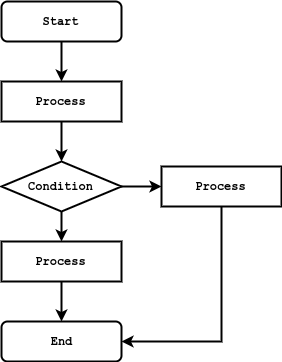
\includegraphics[scale=0.6]{figures/2018052701.png}
    \caption{フローチャート図}
    \label{fig:flowchart}
  \end{center}
\end{figure}

\subsection{データの流れモデルとは}

プロセス (データを処理するプロセス) 間のデータの流れをモデル化したグラフ表現で, データの入出力について, 主に「外部実体 (長方形)」, 「プロセス (丸)」, 「データの流れ (矢印)」, 「ファイル (二つの矢印と平行線)」という 4 つの構成要素で表現している. データの流れ図においては, プロセスの制御やデータのやり取りの方向やタイミングについては表現されていない. データフローチャート図について, 図\ref{fig:dataflowchart} に示す.

\begin{figure}[htbp]
  \begin{center}
    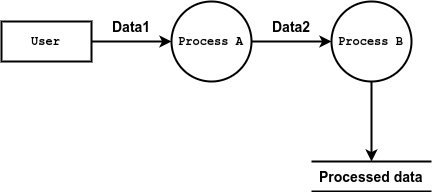
\includegraphics[scale=0.6]{figures/2018052702.png}
    \caption{データフローチャート図}
    \label{fig:dataflowchart}
  \end{center}
\end{figure}

\subsection{フローチャートとデータの流れモデルの差異}

フローチャートは処理手順 (プロセス) の流れを表すグラフとなっており, プロセス間の関連性を認識することが出来るが, どのようなデータが流れているかについては把握することは出来ない. 対して, データの流れモデルにおいては, データを処理するプロセス自体は抽象化され把握は難しいが, 対象のプロセスにどのようなデータが入るのか, またどのようなデータが次のプロセスに渡されるのかついて把握することが出来る.

これらの差異は, フローチャートとデータの流れモデルの優劣を判断するものではなく, 単にそれぞれ何を主体にするのかが異なっているだけでなので, 何を (プロセス制御の流れなのか, データの流れなのか) 主体としてモデル化するかによって使い分けることが重要である.

\end{document}
